\documentclass{article}

%设置页边距
\usepackage{float}
\usepackage{geometry}
%\usepackage{fancybox}
\usepackage{tikz}
\usepackage{graphicx}
\usetikzlibrary{arrows,positioning}

\geometry{left=2cm,right=2cm,top=2cm,bottom=2cm}

%插入代码
\usepackage{titlesec}
\usepackage{listings}
\usepackage{xcolor}
\lstset{
    numbers=left,
    numberstyle=\scriptsize,
    keywordstyle=\color{red!80},
    commentstyle=\color{red!50!green!50!blue!50}\bf,
    frame=trbl,
    rulesepcolor=\color{red!20!green!20!blue!20},
    backgroundcolor=\color[RGB]{245,245,244},
    escapeinside=``,
    showstringspaces=false,
    xleftmargin=5em,xrightmargin=5em,
    aboveskip=1em,
    framexleftmargin=2em,
}
%\begin{lstlisting}[language=C++]
%\end{lstlisting}

%设置中文
\usepackage{ctex}
\usepackage{algorithm}  
\usepackage{algpseudocode}  
\usepackage{amsmath}  
\renewcommand{\algorithmicrequire}{\textbf{Input:}}  % Use Input in the format of Algorithm  
\renewcommand{\algorithmicensure}{\textbf{Output:}} % Use Output in the format of Algorithm  

\begin{document}
%\begin{CJK*}{UTF8}{gbsn}

\title{091M4041H - Algorithm Design and Analysis\\ [2ex] \begin{large} Assignment 4 \end{large}}
%\title{Assignment 1}


\maketitle

\tableofcontents

\newpage
\section{Linear-inequality feasibility}
Given a set of m linear inequalities on n variables $x_1,x_2,...,x_n$, the \textbf{linear-inequality feasibility problem} asks if there is a setting of the variables that simultaneously satisfies each of the inequalities. 

Show that if we have an algorithm for linear programming, we can use it to solve the linear-inequality feasibility problem. The number of variables and constraints that you use in the linear-programming problem should be polynomial in n and m.


\subsection{Formulation of Linear Programing}
设共有m个线性不等式和n个$x_i$变量$(1\leq i\leq n)$,转化成线性规划问题求解,即对m个线性不等式中每个都增加一个变量$x_j$$(n+1\leq j\leq n+m)$,且$x_j\leq0$,求解目标函数max $\sum-x_j$,若其值为0,则原线性不等式是可满足的。

\begin{center}
max $\sum-x_j$\\
s.t. $\sum_ia_{i}x_i -x_j \leq b_j$\\
$x_i \geq 0$\\
$x_j \geq 0$\\
\end{center} 



\newpage
\section{Interval Scheduling Problem}
A teaching building has m classrooms in total, and n courses are trying to use them. Each course $i (i = 1,2,... ,n)$ only uses one classroom during time interval $[S_i,F_i) (F_i > S_i > 0)$. Considering any two courses can not be carried on in a same classroom at any time, you have to select as many courses as possible and arrange them without any time collision. For simplicity, suppose 2n elements in the set $\{S_1,F_1,... ,S_n,F_n\}$ are all different.

Please use ILP to solve this problem, then construct an instance and use GLPK or Gurobi or other similar tools to solve it.



\subsection{Formulation of Linear Programing}
设$x_i$表示第i门课是否选择,选择为1,否则为0,将$S_1,F_1,...,S_n,F_n$排序使得一天的课程时间被划分为2n-1个区间$T_1,...,T_{2n-1}$,用$N_k$表示一门课所占用的所有区间,使得所有选中课所占的相同总区间个数小于m,即相同时间的课程不多于m个。

\begin{center}
max $\sum_{i=1}^nx_i$\\
s.t. $\sum_{i\in N_k}x_i \leq m$\\
$x_i \in \{0,1\}$, for all i = 1,2,...,n
\end{center} 

\subsection{Soving by GLPK}
\begin{figure}[h]
	\centering
	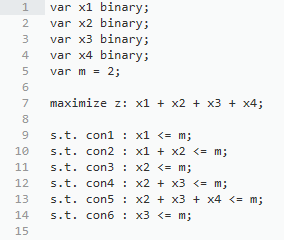
\includegraphics[width=0.4\linewidth]{problem2mod.png}
	\caption{problem2.mod} 
	%\label{fig:mcmthesis-logo}   
\end{figure}

\begin{figure}
	\centering
	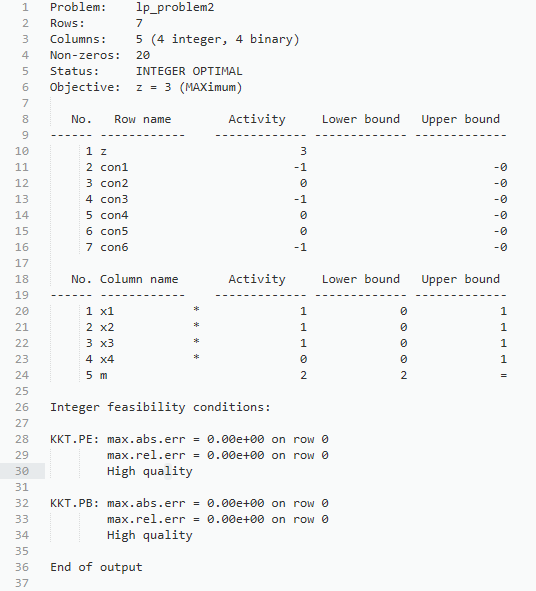
\includegraphics[width=0.7\linewidth]{problem2sol.png}
	\caption{problem2.sol} 
	%\label{fig:mcmthesis-logo}   
\end{figure}

\newpage
\section{Gas Station Placement}
Let's consider a long, quiet country road with towns scattered very sparsely along it. Sinopec, largest oil refiner in China, wants to place gas stations along the road. Each gas station is assigned to a nearby town, and the distance between any two gas stations being as small as possible. Suppose there are n towns with distances from one endpoint of the road being $d_1,d_2,... ,d_n$. n gas stations are to be placed along the road, one station for one town. Besides, each station is at most r far away from its correspond town. $d_1,...,d_n$ and r have been given and satisfied $d_1 < d_2 < ... < d_n, 0 < r < d_1 and d_i + r < d_{i+1} - r$ for all i. The objective is to find the optimal placement such that the maximal distance between two successive gas stations is minimized.

Please formulate this problem as an LP.




\subsection{Formulation of Linear Programing}
设$x_i$表示加油站与路起始点的距离,目标函数为最小化所有加油站间最大距离。加油站与城镇的距离小于r,$x_i$应落在城镇半径为r的区间内,且$x_i$应大于0。

\begin{center}
min max\{$x_{i+1}-x_i$\} i = 0,1,...,n\\
s.t. $x_i - d_i \leq r$\\
$d_i - x_i \leq r$\\
$x_i \geq 0$
\end{center} 


\newpage
\section{Stable Matching Problem }
n men $(m_1,m_2,... ,m_n)$ and n women $(w_1,w_2,... ,w_n)$, where each person has ranked all members of the opposite gender, have to make pairs. You need to give a stable matching of the men and women such that there is no unstable pair. (A matching is unstable if: there is an element A of the first matched set which prefers some given element B of the second matched set over the element to which a is already matched, and B also prefers A over the element to which B is already matched.) Please choose one of the two following known conditions, formulate the problem as an ILP, construct an instance and use GLPK or Gurobi or other similar tools to solve it. 

1. You have known that for every two possible pairs (man $m_i$ and woman $w_j$, man $m_k$ and woman $w_l$), whether they are stable or not. If they are stable, then $S_{i,j,k,l} = 1$; if not, $S_{i,j,k,l} = 0$. $(i,j,k,l \in \{1,2,... ,n\})$

2. You have known that for every man $m_i$, whether $m_i$ likes woman $w_j$ more than $w_k$. If he does, then $p_{i,j,k} = 1$; if not, $p_{i,j,k} = 0$. Similarly, if woman $w_i$ likes man $m_j$ more than $m_k$, then $q_{i,j,k} = 1$, else $q_{i,j,k} = 0$. $(i,j,k \in \{1,2, ... ,n\})$



\subsection{Formulation of Linear Programing}
1.设$x_{ij}$表示$man_i$与$women_j$是否彼此喜欢,若是则为1,否则为0。对于一个男人,他只能选择所有女人中的一个,对于一个女人,她也只能选择所有男人中的一个。若$x_{ij}$与$x_{kl}$同时为1,则$S_{i,j,k,l}=1$,若$x_{ij}$与$x_{kl}$中有且仅有一个为1,则$S_{i,j,k,l}=1$仍旧稳定,当$x_{ij}$与$x_{kl}$同时为0时,$S_{i,j,k,l}$可能为1或0。因此可以总结如下

\begin{center}
min 0\\
s.t. $\sum_{i=1}^nx_{ij} = 1$\\
$\sum_{j=1}^nx_{ij} = 1$\\
$x_{ij}+x_{kl} \leq S_{i,j,k,l}+1$\\
$x_{ij} \in \{0,1\}$
\end{center} 


2.当$p_{i,j,l},p_{j,i,l}$均为1时,$x_{ij}=1$,$x_{kl}=0/1$,当$p_{i,j,l},p_{j,i,l}$均为0时,$x_{ij}=0$,$x_{kl}=0/1$, 当$p_{i,j,l}=1,p_{j,i,l}=0$时,$x_{ij}=1$,$x_{kl}=0/1$,当$p_{i,j,l}=0,p_{j,i,l}=1$时,$x_{ij}=0$,$x_{kl}=0/1$。因此可以总结如下

\begin{center}
min 0\\
s.t. $\sum_{i=1}^nx_{ij} = 1$\\
$\sum_{j=1}^nx_{ij} = 1$\\
$x_{ij}+x_{kl} \leq 3- p_{i,j,l}- p_{j,i,l}$\\
$x_{ij} \in \{0,1\}$
\end{center} 

\subsection{Soving by GLPK}
\begin{figure}
	\centering
	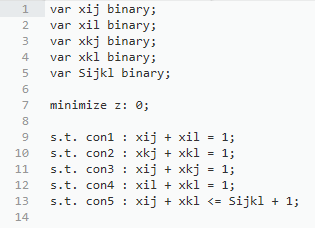
\includegraphics[width=0.4\linewidth]{problem4_1mod.png}
	\caption{problem4\_1.mod} 
	%\label{fig:mcmthesis-logo}   
\end{figure}

\begin{figure}
	\centering
	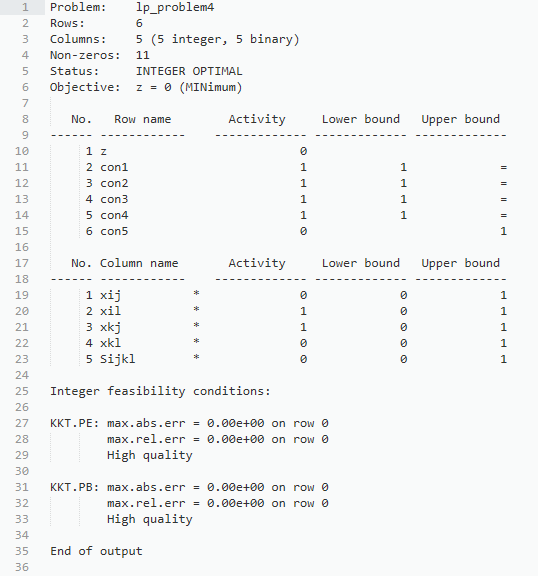
\includegraphics[width=0.7\linewidth]{problem4_1sol.png}
	\caption{problem4\_1.sol} 
	%\label{fig:mcmthesis-logo}   
\end{figure}

\begin{figure}
	\centering
	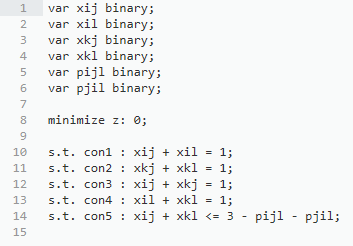
\includegraphics[width=0.4\linewidth]{problem4_2mod.png}
	\caption{problem4\_2.mod} 
	%\label{fig:mcmthesis-logo}   
\end{figure}

\begin{figure}
	\centering
	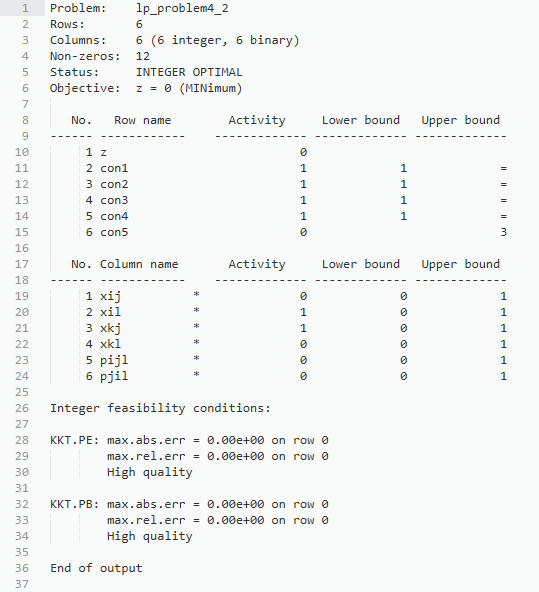
\includegraphics[width=0.7\linewidth]{problem4_2sol.png}
	\caption{problem4\_2.sol} 
	%\label{fig:mcmthesis-logo}   
\end{figure}


\newpage
\section{Duality}
Please write the dual problem of the MultiCommodityFlow problem in Lec8.pdf, and give an explanation of the dual variables. 

Please also construct an instance, and try to solve both primal and dual problem using GLPK or Gurobi or other similar tools.



\subsection{Formulation of Linear Programing}

primal:

\begin{center}
max 0\\
s.t.$\sum_{i=1}^kf_i(u,v) \leq c(u,v)$ \\
$\sum_{v,(u,v)\in E}f_i(u,v) - \sum_{v,(v,u)\in E}f_i(v,u)=0$\\
$\sum_{v,(s_i,v)\in E}f_i(s_i,v) - \sum_{v,(v,s_i)\in E}f_i(v,s_i)=d_i$\\
$f_i(u,v) \geq 0$
\end{center} 

duality:
用$x_{uv}$代表第一条约束,$y_{iu}$代表第二,三条约束:
\begin{center}
min $ c(u,v)x_{uv}+d_iy_{is_i}$\\
s.t. $x_{uv}+y_{iu}-y_{iv} \geq 0$\\
$x_{ut_i}+y_{iu} \geq 0$\\
$x_{t_iv}-y_{iv} \geq 0$\\
$x_{uv} \geq 0$
\end{center} 


\newpage
\section{Dual Simplex Algorithm}
For the problem

minimize

\begin{center} 
$-7x_1 + 7x_2 - 2x_3 - x_4 - 6x_5$
\end{center}

subject to:

\begin{center}
$3x_1 - x_2 + x_3 - 2x_4 = -3$ \\ 
$2x_1 + x_2 + x_4 + x_5 = 4$ \\
$- x_1 + 3x_2 - 3x_4 + x_6 = 12$ \\
$x_i \geq 0,(i = 1,...,6)$
\end{center}

Implement dual simplex algorithm with your favorate language to solve this problem, and make comparison result with GLPK or Gurobi or other similar tools.


\subsection{Formulation of Linear Programing}
对偶方程可表示为
\begin{center}
max $-3y_1 + 4y_2 + 12y_3$\\
$3y_1 + 2y_2 - y_3 \leq -7$\\
$-y_1 + y_2 + 3y_3 \leq 7$\\
$y_1 \leq -2$\\
$-2y_1 + y_2 -3y_3 \leq -1$\\
$y_2 \leq -6$\\
$y_3 \leq 0$
\end{center}

\subsection{Soving by GLPK}
\begin{figure}[h]
	\centering
	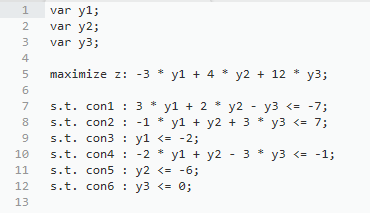
\includegraphics[width=0.5\linewidth]{problem6mod.png}
	\caption{problem6.mod} 
	%\label{fig:mcmthesis-logo}   
\end{figure}

\begin{figure}[h]
	\centering
	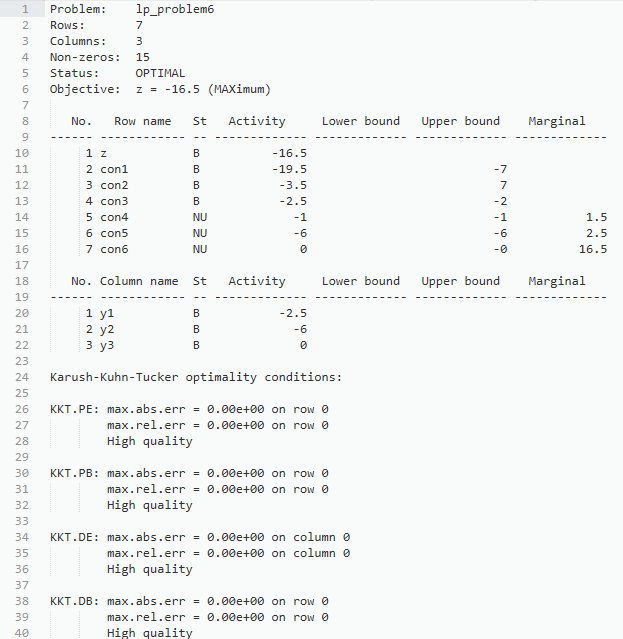
\includegraphics[width=0.8\linewidth]{problem6sol.png}
	\caption{problem6.sol} 
	%\label{fig:mcmthesis-logo}   
\end{figure}


%\end{CJK*}
\end{document}
